\subsection{内存分配}

内存的分配方式与之后的内存释放息息相关,好的分配方式会使得效率大大提高。
根据内存的大小来划分内存如何使用,预计使用32KB用于内存分配的管理空间,
则共有4000组左右的内存用于分配给各个程序使用。

每一组内存经过初始化都拥有自己的数据结构,
即每一组空闲内存的地址和大小都被记录到空闲内存表free。

\begin{table}[!ht]
  \centering
  \begin{tabular}{|c{4cm}|c{8cm}|}
    \hline 
    组号 & 地址 \\
    \hline 
    1 & 0x00003000 \\ 
    \hline 
    2 & 0x00004000 \\
    \hline 
    3 & 0x00005000 \\
    \hline
  \end{tabular}
  \caption{表格示例}
  \label{tab:hello}
\end{table}

一旦系统接收到程序申请内存的请求(需求的内存大小),
就开始在内存中寻找足够大的内存完成这次申请,并返回可供使用的空闲内存的地址。
完成申请后系统需要重新整理空闲内存表free,将最大可用内存组数减一,
将返回给程序空闲空间大小根据程序需求进行调整,并对剩余的可用内存表进行整理。

\begin{listing}[H]
  \inputminted[tabsize=2, firstline=68, lastline=78,
  linenos=true]{c}{../ZOS/src/kernel/memory.c}
\end{listing}

\newpage
\subsection{内存释放}

为保证磁盘空闲空间尽可能少的碎片化,内存释放首先考虑的是使待释放空间与附近空闲空间进行合并。

具体分为三种情况:

\begin{description}
\item[前端空闲:]释放内存的相连前端是空闲内存或释放内存相连两端都是空闲内存
\item[后端可用:]释放内存的相连后端是空闲空间
\item[前端后端均不可用:]挪动空闲空间以合并
\end{description}

已知:待释放的空间的地址和空间大小

根据空闲内存表free的编号查找地址大于待释放空间的空闲内存,
并根据得到的空闲空间编号及大小区分此时的待释放内存应当采取何种方式释放。
\begin{listing}[H]
  \inputminted[tabsize=2, firstline=91, lastline=95,
  linenos=true]{c}{../ZOS/src/kernel/memory.c}
\end{listing}

\newpage
前端空闲:

当待释放的空间前方有空闲空间时,将free[i-1]的大小加上释放空间的大小

内存释放前后情况如图\ref{fig:mem0}和图\ref{fig:mem1}所示: 

\begin{figure}[h]
  \centering
  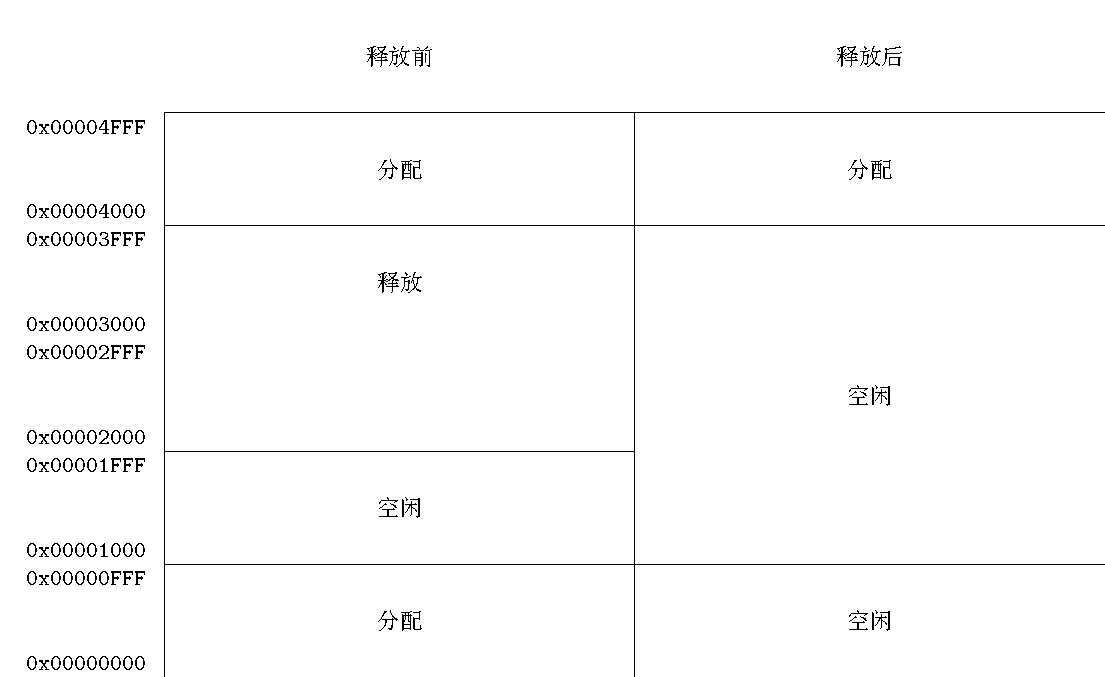
\includegraphics[width=.8\textwidth]{fig/mem0.pdf}
  \caption{前端空闲}
  \label{fig:mem0}
\end{figure}

当待释放的空间后方有空闲空间时,将free[i-1]的大小加上释放空间的大小
\begin{figure}[h]
  \centering
  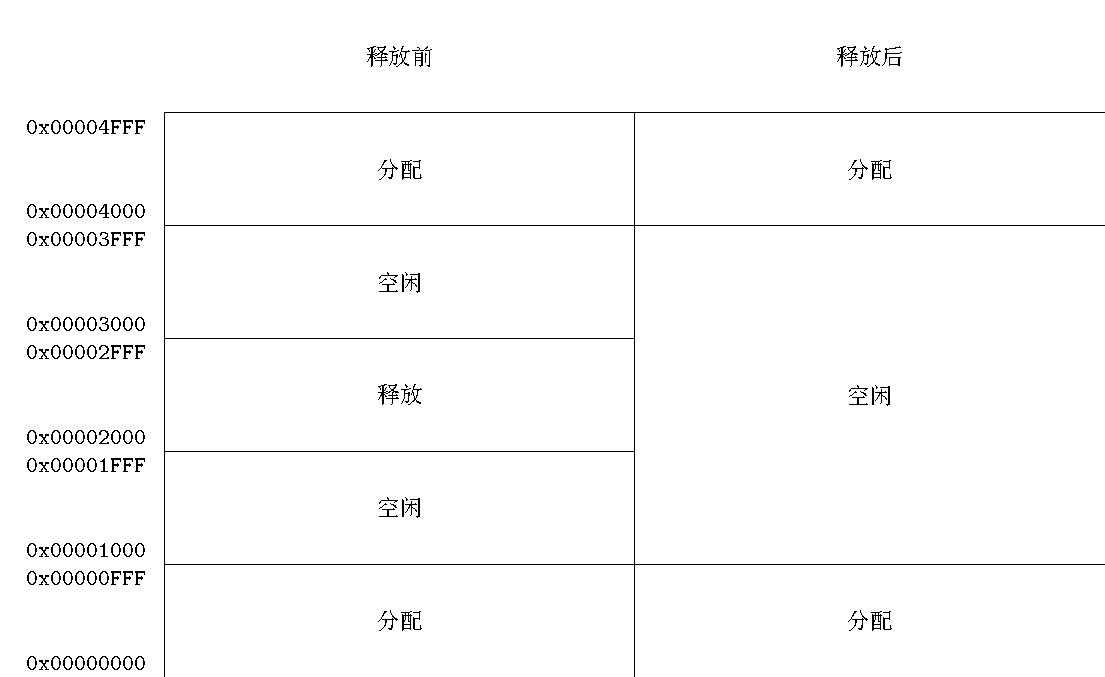
\includegraphics[width=.8\textwidth]{fig/mem1.pdf}
  \caption{前端可用,且后端空闲}
  \label{fig:mem1}
\end{figure}

\newpage
实现如下:

\begin{listing}[H]
  \inputminted[tabsize=2, firstline=98, lastline=116,
  linenos=true]{c}{../ZOS/src/kernel/memory.c}
\end{listing}

\newpage
后端空闲:

内存释放前后情况如图\ref{fig:mem2}所示:

当待释放的空间后方有空闲空间时,将free[i-1]的大小加上释放空间的大小
\begin{figure}[h]
  \centering
  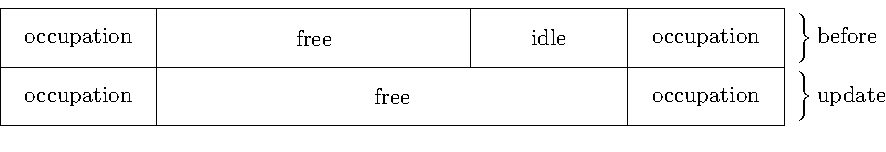
\includegraphics[width=.8\textwidth]{fig/mem2.pdf}
  \caption{后端空闲}
  \label{fig:mem2}
\end{figure}

实现如下:

\begin{listing}[H]
  \inputminted[tabsize=2, firstline=118, lastline=127,
  linenos=true]{c}{../ZOS/src/kernel/memory.c}
\end{listing}

\newpage
前端后端均被占用:

内存释放前后情况如图\ref{fig:mem3}所示:

由于被释放空间周围没有空闲内存,为保证free内各段内存仍然按照内存地址升序排列,
使空闲空间计数最大值加一,free[i]后续空闲内存序号加一,并将释放空间序号定为i。
\begin{figure}[h]
  \centering
  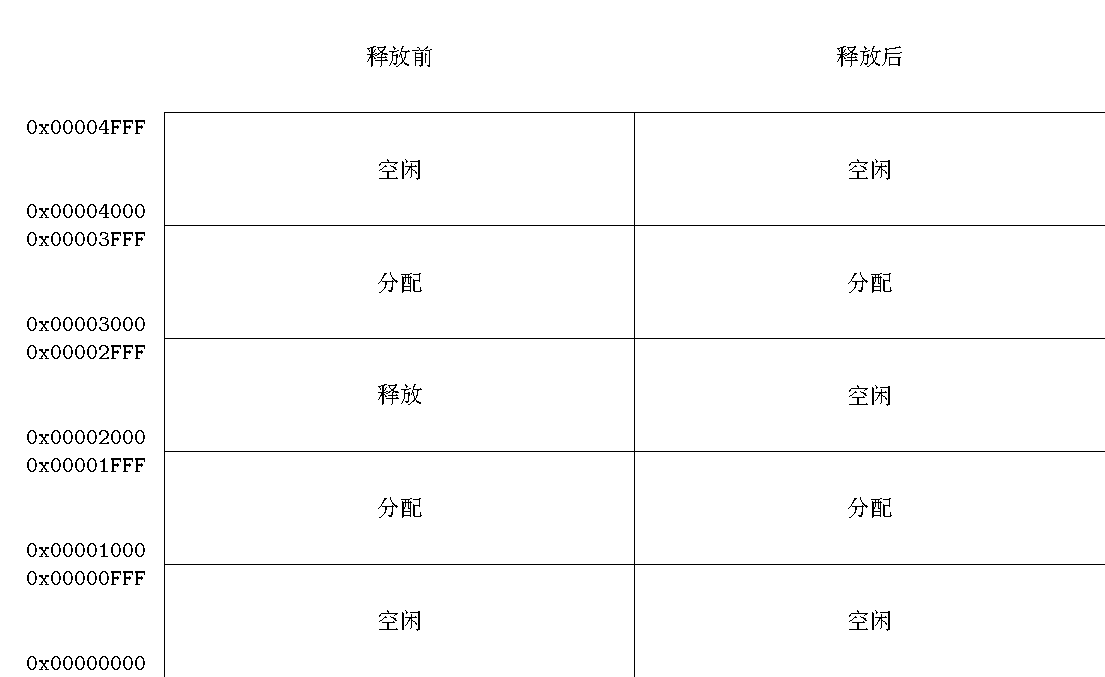
\includegraphics[width=.8\textwidth]{fig/mem3.pdf}
  \caption{前端后端均被占用}
  \label{fig:mem3}
\end{figure}

实现如下:
\begin{listing}[H]
  \inputminted[tabsize=2, firstline=128, lastline=141,
  linenos=true]{c}{../ZOS/src/kernel/memory.c}
\end{listing}